\documentclass[11pt]{article}
\usepackage{amsmath,amssymb,amsthm}
\usepackage[margin=1.1in]{geometry}
\usepackage{tikz}
\usepackage{hyperref}

\theoremstyle{plain}
\newtheorem{theorem}{Theorem}[section]
\newtheorem{lemma}[theorem]{Lemma}
\newtheorem{proposition}[theorem]{Proposition}
\newtheorem{corollary}[theorem]{Corollary}
\theoremstyle{definition}
\newtheorem{definition}[theorem]{Definition}
\theoremstyle{remark}
\newtheorem{remark}[theorem]{Remark}
\theoremstyle{plain}
\newtheorem{conjecture}[theorem]{Conjecture}
\newtheorem{problem}[theorem]{Open Problem}

\newcommand{\tr}{\operatorname{tr}}
\newcommand{\R}{\mathbb{R}}
\newcommand{\F}{\mathbb{F}}
\newcommand{\Om}{\Omega}
\newcommand{\suppop}{\operatorname{ran}}
\newcommand{\suppF}{\operatorname{supp}_{\F}}
\newcommand{\supp}{\operatorname{supp}}
\newcommand{\cJ}{\mathcal{J}}

\title{The Resource Theory of Complexness References\\
in Real Quantum Networks}
\author{Seth Douglas\\[2pt]
{\small ORCID 0009-0007-4708-3252 $\cdot$
\texttt{apsiape@gmail.com}}}
\date{August 2026\\[2pt]
{\small doi:10.5281/zenodo.21907063}}

\begin{document}
\maketitle

\begin{abstract}
Real quantum theory with independent sources cannot reproduce
certain complex network correlations; the known remedy is the
shared two-rebit state $\Om = \tfrac14(I-J\otimes J)$, the
reference frame of complexness of Weilenmann, Gisin, and Sekatski.
We develop the resource theory in which $\Om$ is the unit. We show
that two exact edge self-tests at one source do not fix a single
frame; for commuting induced complex structures the missing datum
is one binary observable, of whose $+1$ sector $\Om$ is the
normalized projector. The partial references
$\eta_t = \tfrac14(I - tJ\otimes J)$, $0<t<1$, are useful for
$t > t_*\approx 0.708$ yet admit no exact finite-copy conversion
to $\Om$ under stochastic real separable operations with
charge-free ancillas, while distilling $\Om$ under rLOCC at rate
at least one. Every resource on $m$
separated holders carries a transpose-charge code
$H(\sigma)\le\F_2^m$, non-increasing under real separable
operations with charge-free ancillas; frame-code states realize
every even-weight code, with a maximal reference one-shot
obtainable between holders $a,b$ iff $e_a+e_b$ is a codeword, and
rate zero (in that class) otherwise. Charges can influence
network statistics only if a parity condition holds on the
source--party incidence graph, and, for frame-code resources, used
charges are
reducible to the weight-2 unit by two mechanisms we keep separate
--- partition coarsening, and activation consuming declared
pairwise auxiliaries --- the frame-sector transcription of the
unlocking and activation of multipartite bound entanglement. All statements are relative to a declared
separable-source-independence axiom.
\end{abstract}

\section{Introduction}

Renou et al.\ \cite{renou2021} showed that quantum theory over the
real numbers, composed with independent sources, is experimentally
falsifiable: certain network correlations of complex quantum
theory are unreachable by any real model whose sources are
uncorrelated (classically correlated sources do not help, by
linearity of their witness), a separation realized experimentally
\cite{li2022,chen2022}. Weilenmann, Gisin, and Sekatski
\cite{wgs2025} identified the exact remedy: a shared two-rebit
state
\[
\Om = \tfrac14\,(I - J\otimes J),
\qquad
J = \begin{pmatrix}0&-1\\1&0\end{pmatrix},
\]
locally invisible (we abbreviate the authors WGS), whose
$m$-party extension restores the full
simulating power of complex theory via the realification of
McKague, Mosca, and Gisin \cite{mckague2009}; one rebit of
inter-source entanglement is necessary and sufficient at the ideal
point. They name the resource a \emph{reference frame of
complexness}; we adopt the contraction \emph{complexness
reference}. A debate has developed around the composition axiom:
Hoffreumon and Woods \cite{hoffreumon2025,hoffreumon2026} argue
the gap closes under an operational notion of independence, and
Barrios Hita et al.\ \cite{barrios2026} give a consistent real
description in a related spirit, while Feng, Ren, and Vedral
\cite{feng2025} and Moradi Kalarde, Xu, and Renou
\cite{kalarde2026} defend the separation, and Y\={\i}ng et al.\
\cite{ying2025} reframe the question through foil theories.
Multipartite aspects of the gap are studied in \cite{sarkar2025};
the two-rebit skew sector is isolated as ``tomographically
nonlocal'' entanglement in \cite{baldijao2026}, whose multipartite
structure is, to our knowledge, open. There is no tension between
our results and the single-scenario uselessness theorems of
\cite{baldijao2026}: the resourcefulness studied here is a network
phenomenon, relative to a declared source-independence axiom.

This paper develops that multipartite structure as a resource
theory with $\Om$ as its unit. We state the honest relation to
prior work at the outset. Once the transpose-sector decomposition
is written down, our objects are stabilizer-like states in the
$\sigma_y$ sector: the family we study generalizes states of
Wootters \cite{wootters2012}, is contained in the unlockable
stabilizer class of Wang and Ying \cite{wangying2007}, and our
four-source activation construction is the frame-sector
transcription of the Smolin-state unlocking
\cite{smolin2001,augusiakhorodecki2006} and of multiparticle
activation \cite{hhh1999,durcirac2000,durcirac2000b,sst2003}. What
this paper adds is the resource theory built on that transfer: a
subgroup-valued monotone (the transpose-charge code) with a weight
obstruction; an exact per-pair distillability dichotomy graded by
the code, where the entanglement-theoretic ancestors give binary
classifications; a graded hierarchy of partial references with a
finite-copy/asymptotic separation; a parity law for which charges
can influence network statistics at all; and the complexness (not
entanglement) reading of all of it --- the states in question are
complex-separable, so no statement here is about ordinary
entanglement. The proof mechanisms also have ancestors, used
gratefully: sector preservation is a modes-of-asymmetry argument
\cite{marvian2014} for an antiunitary symmetry, whose
reference-frame treatment is \cite{gour2009}; bipartite transpose
covariance appears in \cite{kondra2023} within the imaginarity
resource theory \cite{hickeygour2018,wu2021prl,wu2021pra,wu2024},
from whose monotones we differentiate ours in
\S\ref{sec:imagcompare}; the structural roots are bilocal
tomography \cite{hardy2012} and real entanglement geometry
\cite{cfr2001}.

One terminological caution. The WGS reference state is real-QT
entangled across every bipartition, and that real entanglement is
undistillable by real LOCC precisely because its complexification
is separable \cite{wgs2025}; it carries no ordinary entanglement
at all. Bound \emph{real entanglement} and bound
\emph{complexness} (zero distillability of the reference itself)
are different notions, and this paper concerns the latter.

\section{Setting}\label{sec:setting}

\paragraph{Notation.} A \emph{rebit} is $\R^2$ with real density
matrices (PSD, symmetric, unit trace) and real symmetric effects.
Real CP maps are $\Phi(X) = \sum_k A_kXA_k^{\mathsf T}$; channels
satisfy $\sum_kA_k^{\mathsf T}A_k = I$, and single terms without
the normalization are stochastic branches. $X, Y, Z$ are the
Paulis; on a real carrier $Y = iJ$ is not a real operator while
$J$ is. $V := \mathrm{diag}(1,-1)$ denotes the reflection,
$VJV^{\mathsf T} = -J$. Bell states are
$|\Phi^\pm\rangle = \tfrac1{\sqrt2}(|00\rangle\pm|11\rangle)$,
$|\Psi^\pm\rangle = \tfrac1{\sqrt2}(|01\rangle\pm|10\rangle)$.
$e_a\in\F_2^m$ is the indicator vector of holder $a$; $|c|$ is
Hamming weight, $\supp(c) = \{i : c_i = 1\}$, $|c\wedge c'|$
counts common support, and $d(C) = \min\{|c| : c\in C,\,c\neq0\}$
for a code $C\neq\{0\}$. $\partial$ denotes the $\F_2$ boundary
map of a graph (edges to vertex parities). For an operator $\rho$,
$\suppop\rho$ is its range; charge supports $\suppF$ are defined
in \S\ref{sec:code}.

\paragraph{Free scenario.} Sources $S_1,S_2,\dots$ each distribute
subsystems to subsets of parties; parties measure jointly on what
they receive, in a \emph{single round}: sources emit, settings are
drawn, parties measure and output. There is no communication
within a round and no preparation stage. \emph{Free models}
satisfy \textbf{separable source independence}: conditioned on
shared classical randomness $\lambda$, the joint source state is a
product $\rho_{S_1}^\lambda\otimes\rho_{S_2}^\lambda\otimes\cdots$
(arbitrary internal source entanglement); all states, effects, and
processing are real. This class is the convex hull of the
strictly-independent class of \cite{renou2021}; any witness linear
in the observed correlation retains its strictly-independent bound
over it (we use this twice below). A correlation is \emph{nonfree}
if it is realizable in complex quantum theory with independent
sources but by no free real model.

\paragraph{Resource-assisted realizations.} A \emph{resource} is
an additional real state $\eta$ whose subsystems (\emph{shares})
are assigned to holders (sources or parties) --- the assignment,
the \emph{partition} $\mathcal P$, is part of the embedding data.
When the network routes several shares to one location, that
location is their holder \emph{ab initio}: partition coarsening is
part of the declared embedding, never an in-protocol quantum
transmission. An
assisted realization may use a \emph{preparation phase} before
settings are drawn, in which holders may measure
\emph{$\eta$-descendants only} (resource shares and their images
under local processing, together with local charge-free ancillas),
broadcast classical outcomes --- broadcasting is a free operation
(the record is classical, though correlated with the surviving
resource) --- and apply local corrections to resource shares. Systems distributed by free sources exist only in-round
and are never touched in preparation; within the round there is no
communication.

\begin{lemma}[No in-round manufacturing]\label{lem:noman}
Free models gain nothing from the structure above: with no
resource, the preparation phase carries only classical randomness,
which the free class already has; and free sources cannot convert
their in-round payloads into shared references.
\end{lemma}

\begin{proof}
The first claim is immediate from the restriction of preparation
measurements to $\eta$-descendants (local charge-free ancillas
yield only local randomness; a preparation phase granted to free
sources would likewise only refine $\lambda$, since measurements
on $\lambda$-conditioned product states generate classical data
already expressible as shared randomness). The second claim is a
closure statement: the free class is, by definition, closed under
arbitrary local real instruments applied in-round by parties ---
parties only produce outputs, and there is no in-round channel
through which a measurement outcome could steer any other
location's operations. Hence no in-round action leaves the class.
\end{proof}

\paragraph{Usefulness.} A resource $\eta$ is \emph{useful} if some
assisted realization exactly produces a nonfree correlation $P$.
No safeguard clause is needed: substituting any free state for
$\eta$ in the realization would exhibit a free realization of $P$
--- impossible. Usefulness is defined without reference to a
partition; boundness (Definition~\ref{def:bound}) is the
partition-relative notion. For \emph{frame-code resources}
(Definition~\ref{def:framecode}), whose states are determined by
their frame characters, the frame twirl of
Definition~\ref{def:walsh} gives a certification handle: the
twirled resource is free, so usefulness certifies that some
nontrivial frame character is doing work
(Theorem~\ref{thm:activation}).

\paragraph{Conversion classes and rates.} For a fixed partition of
$\eta$'s shares among permanently separated holders:
\textbf{rLOCC} is finite-round local real operations and classical
communication; \textbf{rSEP} is the larger real-separable class
$\Lambda(X) = \sum_k(A^{(1)}_k\otimes\cdots\otimes A^{(m)}_k)\,X\,
(A^{(1)}_k\otimes\cdots\otimes A^{(m)}_k)^{\mathsf T}$. In both,
ancillas are \emph{charge-free}: local real states, product across
holders. The distillation rate between holders $a,b$ under class
$\mathcal C$ is
\[
D^{a:b,\mathcal C}_\Om(\sigma)
:= \sup\Bigl\{r : \exists\,\Lambda_n\in\mathcal C,\;
\tfrac12\bigl\|\Lambda_n(\sigma^{\otimes n})
-\Om^{\otimes\lfloor rn\rfloor}\bigr\|_1\to0\Bigr\},
\]
a joint (not per-copy) trace-distance criterion; $D^{a:b}_\Om$
abbreviates the rLOCC rate, and $D_\Om$ the two-holder case. A
stochastic exact conversion with success probability $p>0$,
i.i.d.-repeated and heralded, gives deterministic rate $\ge p$;
we use this silently. \emph{Auxiliary-assisted} conversions,
where declared additional resource states are consumed, appear
in \S\ref{sec:activation} with their accounting stated in each
theorem.

\paragraph{Why $\Om$ is not shared randomness.} In complex quantum
theory $\Om = \tfrac12(|y_+y_+\rangle\langle y_+y_+| +
|y_-y_-\rangle\langle y_-y_-|)$ is a shared classical bit in the
$y$ basis. That ensemble does not exist for the free class: the
states $|y_\pm\rangle\langle y_\pm| = \tfrac12(I\pm iJ)$ are not
real states, and $\Om$ is real-\emph{entangled} --- by the real
concurrence criterion (\S\ref{sec:graded}) it admits no
decomposition into real product states conditioned on any
$\lambda$. The bit is classical only in a description the free
theory cannot express; that representational deficit is exactly
what the resource theory quantifies, and it is operationally
meaningful because it shows up in observable correlations
\cite{renou2021}. Everything below is relative to the declared
axiom; under operational-independence axioms the free class
itself changes \cite{hoffreumon2026}.

\section{What the reference certifies: frame locking}
\label{sec:lock}

An orthogonal complex structure on a real carrier is $\cJ$ with
$\cJ^{\mathsf T} = -\cJ$, $\cJ^2 = -I$; its \emph{frame line} is
$[\cJ] = \{\cJ,-\cJ\}$. Exact two-source self-tests extract, at
the ideal score, the state $\Om$ across the tested edge and an
effective complex structure on each end's support \cite{wgs2025};
all real projective measurements are self-testable
\cite{supic2024}.

\begin{theorem}[Edgewise exactness does not lock the source]
\label{thm:nolock}
There is a resource-assisted configuration --- a four-dimensional
source carrier $S = A\otimes B$ sharing
$\Om_{AC}\otimes\Om_{BD}$ with two neighbor systems $C,D$ --- in
which each edge block runs the exact ideal WGS realization on its
own tensor factor, yet the two induced complex structures
$\cJ_1 = J_A\otimes I_B$ and $\cJ_2 = I_A\otimes J_B$ on the same
full support ($\rho_S = I_{AB}/4$) satisfy $[\cJ_1]\neq[\cJ_2]$.
\end{theorem}

\begin{proof}
$\cJ_1\cJ_2 = J_A\otimes J_B$ has eigenvalues $\pm1$, so
$\cJ_2\neq\pm\cJ_1$, while both are orthogonal complex structures.
Each edge block is the ideal WGS two-source realization on its own
factor, extended by the identity on the spectator factor, which
changes no probability; each edge's ideal score is that of the WGS
construction \cite{wgs2025}.
\end{proof}

\begin{theorem}[Frame locking, commuting case]\label{thm:lock}
Let $\cJ_1,\cJ_2$ be commuting complex structures on a real
carrier and $R := -\cJ_1\cJ_2$, which is real symmetric with
$R^2 = I$. For any orthogonal projection $\Pi$ commuting with
$\cJ_1,\cJ_2$: $[\cJ_1|_\Pi] = [\cJ_2|_\Pi]$ iff
$R\Pi = \nu\Pi$ for some $\nu\in\{\pm1\}$, and explicitly
$R\Pi = \nu\Pi \iff \cJ_2\Pi = \nu\cJ_1\Pi$.
\end{theorem}

\begin{proof}
If $\cJ_2\Pi = \nu\cJ_1\Pi$ then
$R\Pi = -\cJ_1\cJ_2\Pi = -\nu\cJ_1^2\Pi = \nu\Pi$; conversely
multiply $R\Pi = \nu\Pi$ on the left by $\cJ_1$.
\end{proof}

\begin{remark}\label{rem:lockstate}
In the tensor-factor setting of Theorem~\ref{thm:nolock}, where
$\cJ_1\cJ_2 = J_A\otimes J_B$, one has
$\tfrac14(I - \cJ_1\cJ_2) = \tfrac12\Pi_+$: the two-rebit
reference coincides, as an operator on the source carrier $S$,
with the normalized projector (equivalently, the maximally
mixed state) on the $R = +1$ sector --- the reference \emph{is}
the cross-port lock. The $m$-party WGS state
$\rho^{(m)}_W = \tfrac12(Q_+^{\otimes m} + Q_-^{\otimes m})$ with
$Q_\pm = \tfrac12(I\pm iJ)$ is real (the summands are complex
conjugates), PSD and unit trace (the $Q_\pm$ are rank-one
projectors), and has every pair marginal equal to $\Om$
\cite{wgs2025}: edge ideality and the cross-port lock are
simultaneously satisfiable; there is no monogamy obstruction. For
noncommuting $\cJ_1,\cJ_2$ the operator $R$ need not be symmetric
or involutive, and the criterion is simply $\cJ_2 = \pm\cJ_1$ on a
common reducing subspace; a one-bit characterization there is
open.
\end{remark}

\begin{remark}[Local invisibility forces a joint lock]
\label{rem:joint}
$J$ is skew, hence invisible to every local real symmetric
observable (single-time real statistics determine only the
symmetric part of an operator; see the companion manuscript
\cite{companion}); $J\otimes J$ is symmetric and jointly
measurable. The lock datum is intrinsically cross-port: real
quantum theory is bilocally but not locally tomographic
\cite{hardy2012}, and the lock is a bilocal datum. Local
indistinguishability of exactly such state families underlies
Wootters' information-hiding analysis \cite{wootters2012}.
\end{remark}

\begin{lemma}[Transpose-flag structure; restated from
\cite{liu2026}]\label{lem:flag}
In the exact self-testing normal form of Liu et al.\
\cite{liu2026}, certified observables satisfy $\widehat X\mapsto
X\otimes I$, $\widehat Z\mapsto Z\otimes I$, $\widehat Y\mapsto
Y\otimes Z_{f}$ on a local flag register $f$: only $Y$ sees the
flag, and the flag is the sign of the extracted complex structure
($Y^{\mathsf T} = -Y$ corresponds to $\cJ\mapsto-\cJ$ under
realification). With $K = XX - YY + ZZ$ measured using the literal
same certified operators,
$K_+ = 4|\Phi^+\rangle\langle\Phi^+| - I$ (spectrum
$\{3,-1,-1,-1\}$) and $K_- = 2F_{\mathrm{swap}} - I$ (spectrum
$\{1,1,1,-3\}$, $F_{\mathrm{swap}}$ the two-qubit swap), the flag
product commutes with $K$ and
$\Pr[f_1\neq f_2]\le\tfrac{3-\langle K\rangle}2$; Liu et al.\
prove this and chain it along a line of parties.
\end{lemma}

\begin{remark}
Two observations are ours. Without literal operator reuse the
lemma fails: two independently certified triples give ideal scores
with uncorrelated flags. And $K$ synchronizes \emph{signs} between
already-identified carriers; it cannot merge distinct
tensor-factor complex structures, which requires the support
condition of Theorem~\ref{thm:lock}.
\end{remark}

\begin{conjecture}[Routed connected-graph rigidity]
\label{conj:routed}
Define the \emph{source-interaction graph}: one vertex per source,
an edge when some party receives systems from both. Assume (A1)
every edge supports an exact WGS block (three distinct parties; a
source-interaction graph alone does not suffice --- two sources
feeding one party form a tree whose every correlation is trivially
real-simulable); (A2) each edge self-test's effective complex
structure on a source's support acts on a common logical carrier,
with commuting induced structures across ports, and is the
structure entering teleported $K$-tests supplied by
source-internal Bell links between that source's receiving
parties. Then for connected source-interaction graphs there is a
single correlation, generated from complex product sources, whose
exact real simulations force frame synchronization on every edge
and reduce the assisting resource to $\rho^{(m)}_W$ under real
local operations. Expected mechanism: port locks propagate flag
equality along the line graph, which is connected whenever the
graph is; acyclicity plays no role. No later section depends on
this conjecture.
\end{conjecture}

\section{The graded layer: partial references}\label{sec:graded}

\begin{definition}\label{def:eta}
$\eta_t := \tfrac14(I - t\,J\otimes J)$ for $t\in[0,1]$;
$\eta_1 = \Om$, $\eta_0 = I/4$, and
$\tr[\eta_t(J\otimes J)] = -t$. By the real-concurrence formula
$C_\R(\rho) = |\tr(\rho\,J\otimes J)|$ for two-rebit states, which
vanishes iff $\rho$ is real-separable \cite{cfr2001}, $\eta_t$ is
real-entangled iff $t>0$.
\end{definition}

\begin{theorem}[Usefulness above threshold]\label{thm:etauseful}
Let $B_\R = 7.6605$ denote the numerical upper bound of
\cite{renou2021} on the Renou functional over real models with
independent (hence, by convexity, classically correlated) sources
--- a certified hierarchy bound, not an exact constant. Let $P_t$
be the Renou two-source correlation with exactly one deformation:
Alice's third input becomes the POVM $\tfrac12(I\pm tY)$; both
sources, Alice's other inputs, and Charlie's six observables are
unchanged. Then the ideal complex value of the functional at
$P_t$ is $2\sqrt2\,(2+t)$, which exceeds $B_\R$ iff
$t > t_* := \tfrac{B_\R}{2\sqrt2} - 2 \approx 0.7084$; and $P_t$
is exactly realized by a real model assisted by one copy of
$\eta_t$, whose two shares $\alpha$ (Alice) and $\gamma$ (Charlie)
realify the deformed $Y$'s. Hence $\eta_t$ is useful for
$t > t_*$; whether some $\eta_t$-enabled correlation is nonfree
for $t\le t_*$ is open.
\end{theorem}

\begin{proof}[Proof sketch]
Per Bob outcome, the Renou functional is a sum of one CHSH block
in $(A_1,A_2;C_1,C_2)$ and two CHSH blocks pairing $A_3$ with
$A_1$ and $A_2$ respectively (settings $C_3,C_4$ and $C_5,C_6$).
$P_t$ is defined by keeping the ideal Renou settings fixed and
deforming only the $A_3$ POVM, so every correlator is linear in
$t$: the first block keeps its ideal value $2\sqrt2$, and in each
$A_3$ block the two $A_3$-correlators (jointly worth $\sqrt2$ at
the ideal settings) scale by $t$ while the two others (worth
$\sqrt2$) are unchanged, giving $\sqrt2(1+t)$ per block and
$2\sqrt2 + 2\cdot\sqrt2(1+t) = 2\sqrt2(2+t)$ in total (at $t=1$,
the complex maximum $6\sqrt2$). For the assisted realization:
Alice realifies her deformed measurement as the real observable
$J_{\mathrm{sys}}\otimes J_\alpha$ and Charlie realifies each $Y$
in his observables through $J_{\mathrm{sys}}\otimes J_\gamma$;
single-$Y$ correlators vanish on both sides (frame marginals
maximally mixed; Bell states carry no single-$Y$ moment), $X$- and
$Z$-correlators are unchanged, and every $YY$ correlator matches
with the correct sign: $Y\otimes Y = -\,J\otimes J$ on the system
pair, and the realified correlator carries the additional frame
factor $\tr[\eta_t\,J_\alpha J_\gamma] = -t$, so
$\langle Y\otimes Y\rangle_{\mathrm{complex,deformed}} =
t\,\langle Y\otimes Y\rangle_{\mathrm{ideal}}$ is reproduced term
by term across all Bob outcomes.
\end{proof}

\begin{theorem}[No exact finite-copy conversion]\label{thm:noexact}
For $0<t<1$ and every finite $n$, no stochastic real separable
operation with charge-free ancillas maps $\eta_t^{\otimes n}$ to
$\Om$ exactly. Moreover every $n = 1$ separable branch has
normalized output $\sigma$ with
$\tfrac12\|\sigma-\Om\|_1\ge(1-t)/2$; the fixed-accuracy question
for $n>1$ is open (the rate statement below shows the gap closes
as $n\to\infty$).
\end{theorem}

\begin{proof}
\emph{Support half.} $\suppop\Om =
\mathrm{span}_\R\{|\Phi^-\rangle,|\Psi^+\rangle\}$; the vector
$a|\Phi^-\rangle + b|\Psi^+\rangle$ has coefficient matrix
$\tfrac1{\sqrt2}\begin{pmatrix}a&b\\b&-a\end{pmatrix}$ of
determinant $-(a^2+b^2)/2$, so the span contains no nonzero real
product vector. Charge-free ancillas decompose into real pure
product states and extend product vectors to product vectors;
discarding a subsystem composes the branch with rank-one
product effects on the discarded factor, re-expanding it into
product-supported terms. Since $\eta_t^{\otimes n}$ is full rank,
every nonzero separable branch $\sum_k(A_k\otimes B_k)(\cdot)
(A_k\otimes B_k)^{\mathsf T}$ has each term supported on
$\operatorname{ran}A_k\otimes\operatorname{ran}B_k$; exact output
$\Om$ forces these product subspaces into $\suppop\Om$ ---
contradiction.
\emph{Gap half ($n = 1$).} Absorb ancillas as above so each Kraus
factor is an effective real $2\times2$ pair $(A_k,B_k)$. From
$A^{\mathsf T}JA = (\det A)J$,
$\tr[\sigma\,(J\otimes J)] = -\tfrac{t}{p}\sum_k\det A_k\det B_k$
with $p = \tfrac14\sum_k\|A_k\|_F^2\|B_k\|_F^2$ (the cross term
$\tr(J\,M)$ vanishes for symmetric $M$), and
$\|A\|_F^2\ge2|\det A|$ gives $|\tr(\sigma\,J\otimes J)|\le t$
while $\tr(\Om\,J\otimes J) = -1$; since $\|J\otimes J\| = 1$,
$\tfrac12\|\sigma-\Om\|_1\ge(1-t)/2$.
\end{proof}

\begin{theorem}[Distillation at unit rate]\label{thm:distill}
For every $t>0$ there is an rLOCC protocol $\Lambda_n$ producing
$m_n = n$ output pairs with
$\tfrac12\|\Lambda_n(\eta_t^{\otimes n}) - \Om^{\otimes n}\|_1
\to 0$; hence $D_\Om(\eta_t)\ge1$.
\end{theorem}

\begin{proof}
Write $\eta_t = \tfrac{1+t}2\Om + \tfrac{1-t}2\bar\Om$ with
$\bar\Om = \tfrac14(I + J\otimes J)$: copy $i$ carries a hidden
branch sign $X_i$, defined as the $J\otimes J$ eigenvalue of its
branch ($X_i = -1$ for $\Om$), i.i.d.\ with
$\Pr[X_i = -1] = \tfrac{1+t}2$. The two
holders measure the commuting real observables
$J^{(1)}\otimes J^{(i)}$ on their local sides ($i = 2,\dots,n$)
and exchange outcomes; the product $w_i$ of the two local parities
equals $X_1X_i$ deterministically given the branches, and the
parity measurements commute with the branch decomposition, so
conditioned on the branch vector the post-measurement
\emph{marginal} of pair $i$ is its branch state. A majority vote
over $\{w_i\}$ estimates $X_1$ with error
$\epsilon_n\le\exp[-(n-1)t^2/2]$; set $\hat X_i = \hat X_1w_i$.
One designated holder applies $V$ to its side of every pair with
$\hat X_i = +1$ (the $\bar\Om$ branch), including pair 1 when
$\hat X_1 = +1$. Conditioned on a correct vote, each pair's
marginal is exactly $\Om$, but the joint conditional state carries
the residual stabilizer group generated by the measured parities:
$h_i = J^{(1)}_AJ^{(i)}_A$ and their $B$-side partners, the latter
products of the $h_i$ with the pair stabilizers, which are
twirl-invariant --- so a group element's character below depends
only on its $h$-content. To kill the residuals, both holders apply
$V\otimes V$ on pair $i$ keyed to an \emph{independent} shared
random bit $b_i$ per pair: each pair's state is fixed
($V\otimes V$ commutes with $\Om,\bar\Om$) while
$h_i\mapsto(-1)^{b_1+b_i}h_i$, so every group element with
nonempty $h$-content averages to zero once the $b_i$ are
discarded; the figure of merit is the $b$-averaged output, which
on the correct-vote branch is exactly $\Om^{\otimes n}$. The
unconditioned output is then within
joint trace distance $\epsilon_n$ of $\Om^{\otimes n}$, with
$m_n = n$ output pairs: rate $\ge1$ is achieved (we expect
equality but prove only the lower bound; the charge code is
non-quantitative, \S\ref{sec:imagcompare}).
\end{proof}

The reference is graded in isolation: one-shot and finite-copy
exact inequivalence coexist with asymptotic equivalence at unit
rate.

\section{The transpose-charge code}\label{sec:code}

\begin{definition}[Charges]\label{def:charge}
Fix a partition of a resource into $m$ holders with an orthogonal
basis on each (the decomposition below is invariant under local
orthogonal, not general invertible, basis changes). Let $T_i$ be
transpose on holder $i$; the commuting involutions $T_i$ split
operators into mutually Hilbert--Schmidt-orthogonal sectors
$\rho = \sum_{c\in\F_2^m}\rho_c$ with
$T_i(\rho_c) = (-1)^{c_i}\rho_c$. Global symmetry of real states
forces even-weight $c$. The \emph{charge support} is
$\suppF(\rho) = \{c:\rho_c\neq0\}$ and the \emph{charge code} is
$H_{\mathcal P}(\rho) = \mathrm{span}_{\F_2}\suppF(\rho)$
(we write $H(\rho)$ when the partition is clear; every statement
below is relative to $\mathcal P$).
\end{definition}

\begin{definition}[Frame characters; twirl]\label{def:walsh}
A \emph{frame resource} carries one rebit per holder. On $m$ frame
rebits let $G_c := \bigotimes_iJ_i^{c_i}$; for even $c$ these are
real symmetric involutions, mutually commuting, with the sign
cocycle $G_cG_{c'} = (-1)^{|c\wedge c'|}G_{c+c'}$, and we write
$\hat\rho(c) := \tr[\rho\,G_c]$ for the frame components of a
resource ($\{G_c\}$ spans the commutative frame algebra, not the
full operator space; for the frame-code states below the
components determine the state). The \emph{frame twirl} applies
independent uniformly random reflections $V$ per rebit; on a frame
resource it kills every $c\neq0$ component and leaves a diagonal,
classically correlated --- hence free --- state. (The twirl frees
\emph{any} resource, but only for frame-code states does twirling
coincide with zeroing all frame characters $\hat\rho(c)$ --- for
general states the twirl also removes non-frame components, so
character bookkeeping certifies usefulness only in the frame-code
setting; this is why Theorem~\ref{thm:activation} and
Corollary~\ref{thm:noirr} are stated for frame-code resources.) In a fixed assisted realization of a
correlation $P$, whose outcome probabilities are linear functionals
$\tr[E\,\rho]$ of the resource operator, a codeword $c$
\emph{contributes} if some such functional changes when the
component $\hat\rho(c)$ is set to zero (linearity licenses
evaluating the functionals off the state space).
\end{definition}

\begin{theorem}[Span monotonicity]\label{thm:span}
For every rSEP protocol $\Lambda$ with charge-free ancillas and
every $n$,
\[
H\bigl(\Lambda(\sigma^{\otimes n})\bigr)\subseteq H(\sigma).
\]
In particular $e_a + e_b\notin H(\sigma)$ implies
$D^{a:b,\mathrm{rSEP}}_\Om(\sigma) = 0$, and approximation cannot
evade the obstruction.
\end{theorem}

\begin{proof}
Each holder-local real CP map commutes with the partial transpose
on its own holder (a global real map commutes only with the global
transpose), so every product Kraus term of an rSEP operation
preserves each charge sector; charge-free ancillas occupy sector
$0$; charges add over tensor factors; and partial trace kills
sectors charged on the discarded holder. Tensor powers therefore
occupy sums of charges, whence the span is the invariant. For the
approximation clause: a vanishing $(a,b)$ weight-2 sector forces
$\tr[\rho(-J_aJ_b)] = 0$ while $\Om$ gives $1$, so
$\tfrac12\|\rho-\Om\|_1\ge\tfrac12$.
\end{proof}

\begin{remark}
Shared entangled ancillas are excluded by hypothesis;
\S\ref{sec:activation} shows they are exactly the doorway of
activation.
\end{remark}

\begin{theorem}[Weight-2 sectors distill]\label{thm:w2}
(i) Every real-entangled two-rebit state has positive rLOCC rate:
independent local $SO(2)$ twirls (which fix $J$) project $\rho$
onto $\tfrac14(I + \zeta\,J\otimes J)$ with
$\zeta = \tr(\rho\,J\otimes J)$; a single-side $V$ when
$\zeta>0$ yields $\eta_{|\zeta|}$, and
$|\zeta| = C_\R(\rho)>0$ by the convex-roof identity of
\cite{cfr2001}; apply Theorem~\ref{thm:distill}. (ii) If
$\rho_{e_a+e_b}\neq0$ (charge support, not merely span), rank-one
real product effects on the other holders --- which annihilate
sectors charged there --- followed by local two-dimensional
projections at $a,b$ (conjugations $\Pi J\Pi$ sweep all rank-two
skew operators) leave, with nonzero probability, a two-rebit state
with nonzero $J\otimes J$ moment --- some choice succeeds, by the
contrapositive: the operators $\Pi J\Pi$ over rank-two projections
$\Pi$ span all skew operators at $(a,b)$, and rank-one real
product effects elsewhere span the symmetric operators there, so
if every choice gave zero moment, the sector $\rho_{e_a+e_b}$
would pair to zero with a spanning family and vanish; hence
$D^{a:b}_\Om(\rho)>0$.
(iii) Consequently, for $m = 2$ with rebit holders no useful
resource has zero rate: charge zero forces $\zeta = 0$, hence real
separability by the converse direction of \cite{cfr2001} --- a
two-rebit theorem, the single load-bearing external input of this
clause --- hence freeness (higher-dimensional two-holder carriers
remain open). For $m = 3$ the
same holds among resources with $H\neq\{0\}$; whether a
charge-zero real-entangled three-holder resource can be useful is
open, as is the regime
$e_a+e_b\in H(\rho)\setminus\suppF(\rho)$.
\end{theorem}

\begin{definition}[Frame-code states]\label{def:framecode}
For an even-weight binary linear code $C\le\F_2^m$ with chosen
generators $g_1,\dots,g_\ell$ and signs $s_j\in\{\pm1\}$, let
\[
\sigma_C := 2^{-m}\prod_{j=1}^\ell(I + s_jG_{g_j}),
\]
a valid state ($\prod_j(I+s_jG_{g_j})$ is $2^\ell$ times a nonzero
projector: independence of the generators keeps $-I$ out of the
generated sign group), with
$H(\sigma_C) = \suppF(\sigma_C) = C$. The signs on non-generator
codewords are induced through the cocycle and depend on the
generating set. For the maximal even-weight code this is, up to
conventions, the family of states of Wootters \cite{wootters2012}
(his Eq.~(22): the real part retains exactly the strings with
evenly many $\sigma_y$'s); as a stabilizer construction the family
lies in the unlockable class of Wang and Ying \cite{wangying2007}.
The arbitrary-code frame reading and the graded classification
below are, to our knowledge, new.
\end{definition}

\begin{theorem}[Per-pair dichotomy]\label{thm:distance}
For every pair $(a,b)$: if $e_a+e_b\in C$, tracing $\sigma_C$ to
$(a,b)$ leaves $\tfrac14(I\pm J_aJ_b)$ --- a maximal reference in
one shot (for the maximal code this recovers Wootters'
simultaneous pairwise maximality \cite{wootters2012}). If
$e_a+e_b\notin C$ then
$D^{a:b,\mathrm{rSEP}}_\Om(\sigma_C) = 0$ for any number of
copies, since $H(\sigma_C^{\otimes n}) = C$ contains no $(a,b)$
weight-2 vector. Corollary: $C$ has no weight-2 codeword iff every
pair has zero rate; $\tau_4 := \tfrac1{16}(I + J^{\otimes4})$ (the
length-4 repetition code, $d = 4$) is the minimal such example in
holder number, since no even-weight code of length $\le3$ avoids
weight-2 words except $\{0\}$; the WGS reference is the maximal
code, all weight-2 sectors present.
\end{theorem}

\begin{remark}[Ordinary entanglement points the other way]
Partial transpose acts on frame-code states as the frame flip
$J_i\mapsto-J_i$, mapping the family to itself, so PPT detects
nothing here. The WGS reference is real-entangled with that
entanglement bound because its complexification is separable
\cite{wgs2025}; $\tau_4$ is likewise complex-separable (a mixture
of even-parity $y$-basis product states). The operative
obstruction for complexness is charge support, not positivity
under the flip.
\end{remark}

\subsection{Relation to imaginarity monotones}
\label{sec:imagcompare}

The imaginarity resource theory
\cite{hickeygour2018,wu2021prl,wu2021pra} takes real states as
free and quantifies $\rho\neq\rho^{\mathsf T}$; its distributed
form \cite{wu2024,kondra2023} studies bipartite scenarios under
real local operations, with scalar monotones such as
$\|\rho-\rho^{T_B}\|_1$ --- the norm of the $T_B$-odd part, which
for the globally symmetric states of this paper is exactly the
$(1,1)$ sector --- and geometric measures. Our objects differ in
three ways. First, every state in this paper is real symmetric,
hence \emph{free} for imaginarity theory; the resource here is
cross-holder structure inside the skew sectors, invisible to any
single-system imaginarity measure. Second, our monotone is
subgroup-valued, not scalar: $H(\sigma)$ records \emph{which}
sectors are occupied, not how much weight they carry, and the
weight obstruction (a code with no weight-2 word never acquires
one under tensor powers and separable processing) has no scalar
counterpart. Third, neither monotone refines the other: the code
is magnitude-blind ($\eta_t$ carries the same code for every
$t>0$, however small), while any scalar sector-weight measure is
support-blind (it cannot record \emph{which} pair carries the
weight, which is exactly what the per-pair dichotomy above turns
on). We are not aware of a prior multipartite sector-support
monotone in either literature.

\section{Visibility, puncturing, activation}
\label{sec:activation}

\begin{figure}[t]
\centering
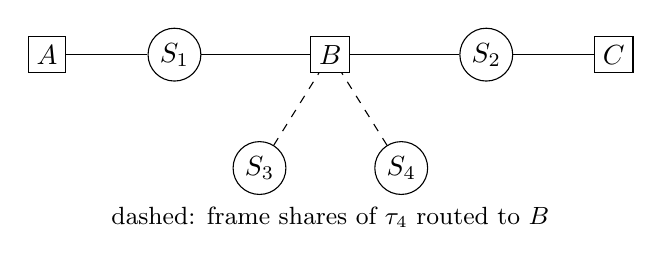
\begin{tikzpicture}[scale=0.9,
  src/.style={draw, circle, inner sep=2pt},
  pty/.style={draw, rectangle, inner sep=3pt}]
\node[src] (S1) at (0,0) {$S_1$};
\node[pty] (A) at (-1.8,0) {$A$};
\node[pty] (B) at (2.2,0) {$B$};
\node[src] (S2) at (4.4,0) {$S_2$};
\node[pty] (C) at (6.2,0) {$C$};
\node[src] (S3) at (1.2,-1.6) {$S_3$};
\node[src] (S4) at (3.2,-1.6) {$S_4$};
\draw (S1) -- (A); \draw (S1) -- (B);
\draw (S2) -- (B); \draw (S2) -- (C);
\draw[dashed] (S3) -- (B); \draw[dashed] (S4) -- (B);
\node at (2.2,-2.3) {\small dashed: frame shares of $\tau_4$
routed to $B$};
\end{tikzpicture}
\caption{The four-source network of Theorem~\ref{thm:abc}.
$S_1,S_2$ run the Renou block through parties $A,B,C$; the
$\tau_4$ shares held by $S_3,S_4$ are routed to $B$, coarsening
the effective holder partition.}
\label{fig:network}
\end{figure}

\begin{theorem}[Charge-flow visibility: necessity]\label{thm:flow}
Attach resource shares to vertices of the \emph{source--party
incidence graph} (vertices: sources and parties; edges: each
transmitted system), many-to-one allowed. Let $q(c)\in\F_2^{V}$ be
the vertex-charge vector, $q_v(c)$ the mod-2 sum of the charges of
$v$'s shares. A charge $c$ can contribute to network statistics
only if $q(c)$ is an $\F_2$-boundary --- $\partial y = q(c)$ for
some edge chain $y\in\F_2^{E}$ --- equivalently, every connected
component contains even total charge.
\end{theorem}

\begin{proof}
Symmetric and skew operators are Hilbert--Schmidt orthogonal, so a
nonzero contraction of the sector-$c$ term against source states
and effects requires each transmitted system to carry a definite
transpose parity $y_e$, with each source state and each effect
forcing even total local parity at its vertex; the resulting
parity assignment is an edge chain $y$ with $\partial y = q(c)$,
and $\operatorname{im}\partial$ over $\F_2$ is exactly the
per-component even-weight vectors.
\end{proof}

\begin{remark}[Converse, with hypotheses]\label{rem:flowconv}
Conversely, when $\partial x = q(c)$ is solvable \emph{and} the
routed $J$-string has even weight on each source's emitted systems
(which is the boundary condition at source vertices), the states
$2^{-k}(I + \delta\,G_{\mathrm{string}})$ ($k$ the number of
systems carrying the routed $J$-string), PSD for
$|\delta|\le1$, realize a network in which $c$ contributes: route
the string along the flow and contract. We use only the $\tau_4$
instance below (Proposition~\ref{prop:abelian}), which is
computed exactly; we do not rely on the general converse.
\end{remark}

\begin{figure}[t]
\centering
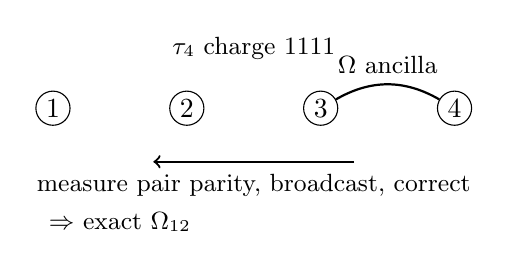
\begin{tikzpicture}[scale=0.85,
  hold/.style={draw, circle, inner sep=1.5pt}]
\node[hold] (h1) at (0,0) {$1$};
\node[hold] (h2) at (2,0) {$2$};
\node[hold] (h3) at (4,0) {$3$};
\node[hold] (h4) at (6,0) {$4$};
\draw[thick] (h3) to[bend left] node[above]
  {\small $\Om$ ancilla} (h4);
\draw[->, thick] (4.5,-0.8) -- (1.5,-0.8);
\node at (3,-1.15) {\small measure pair parity, broadcast,
correct};
\node at (3,0.9) {\small $\tau_4$ charge $1111$};
\node at (1,-1.7) {\small $\Rightarrow$ exact $\Om_{12}$};
\end{tikzpicture}
\caption{Puncturing: pairing charged holders $3,4$ with a declared
$\Om$ ancilla and measuring the pair parities lowers the charge
$1111$ to $1100$, leaving an exact reference on holders $1,2$
after the heralded sign correction.}
\label{fig:puncture}
\end{figure}

\begin{proposition}[Visibility witnessed; frame statistics are
free]\label{prop:abelian}
$\tau_4$ plus two declared $\Om$ ancillas
$\Om_{a_1a_2}\otimes\Om_{a_3a_4}$, with each holder $i$ measuring
$M_i = J_i\otimes J_{a_i}$ (real symmetric, $M_i^2 = I$), yields
exactly $P(x) = \tfrac1{16}(1+x_1x_2x_3x_4)$: weight-4 charge is
not statistically inert. However, statistics generated by frame
characters alone are always freely simulable: the even-$J$ algebra
is commutative, so the outcomes of \emph{all} settings admit one
joint classical distribution, which shared randomness $\lambda$
can sample, each party outputting its sampled values. (Note the
distribution itself can be exotic --- on $\rho^{(3)}_W$ the three
pairwise parities multiply to the operator
$(J_1J_2)(J_1J_3)(J_2J_3) = -I$, impossible for per-source sign
assignments --- but a global $\lambda$-model is not a per-source
sign model, and it suffices.) \emph{Frame characters alone cannot
constitute a nonfree correlation; genuine advantage requires
coupling the character to noncommuting payload.}
\end{proposition}

\begin{lemma}[$\Om$-swap]\label{lem:swap}
On $\Om_{12}\otimes\Om_{34}$, measuring $J_2J_3$ (outcomes
$x = \pm1$, probability $\tfrac12$ each) leaves holders $1,4$ in
exactly $\tfrac14(I + x\,J_1J_4)$.
\end{lemma}

\begin{proof}
Expand $\Om_{12}\otimes\Om_{34} = \tfrac1{16}(I - J_1J_2)(I -
J_3J_4)$ and apply the projector $\tfrac12(I + xJ_2J_3)$; the
terms surviving $\tr_{23}$ are $I$ and
$x\,(J_1J_2)(J_2J_3)(J_3J_4)\propto J_1J_4$ with coefficient
computed via $J^2 = -I$ twice: the conditional state is
$\tfrac14(I + xJ_1J_4)$ at outcome probability $\tfrac12$.
\end{proof}

\begin{theorem}[Puncturing]\label{thm:puncture}
(\emph{$\tau_4$ instance, exact.}) $\tau_4$ plus one declared
$\Om$ ancilla on holders $3,4$, each measuring
$\tfrac12(I + x_iJ_iJ_{a_i})$: the four outcome branches have
probability $\tfrac14$ each and leave holders $1,2$ in exactly
$\tfrac14(I - x_3x_4\,J_1J_2)$ --- the unit up to a heralded,
locally correctable sign. (\emph{General.}) Let $c\in C$ with
$a,b\in\supp(c)$, and pair the (even-sized) set
$\supp(c)\setminus\{a,b\}$ arbitrarily, placing one declared
$\Om$ ancilla on each pair; measure the pair parities
$J_iJ_{a_i}$, $J_jJ_{a_j}$. Then some outcome of nonzero
probability leaves a resource whose $e_a+e_b$ sector is nonzero.
\end{theorem}

\begin{proof}
The $\tau_4$ instance is a direct computation (the cross terms
$x_iJ_i$ alone have odd local charge and vanish; the
$x_3x_4$ term contracts the ancilla's $-J_{a_3}J_{a_4}$ moment).
For the general clause (Figure~\ref{fig:puncture}; ancillas on
non-adjacent holders are obtained along connected paths by
Lemma~\ref{lem:swap}): after the pair measurements, trace out the
holders outside $\{a,b\}$ --- this kills every sector charged
there. The measured observables commute with each other and with
every $G_d\otimes(\text{ancilla strings})$ term, so the
unnormalized conditional $(a,b)$-sector at outcome $x$ is a
well-defined function $f(x)$ of the outcome string. The
codewords $d\in C$ contributing to $f$ are exactly those with
$d_a = d_b = 1$,
$\supp(d)\subseteq\{a,b\}\cup\bigcup(\text{pairs})$, and $d$
restricted to each pair equal to $00$ or $11$; such $d$ is
determined by its set of $11$-pairs, so distinct contributors
carry distinct outcome monomials $\prod_{\text{$11$-pairs}}x_ix_j$
--- linearly independent Walsh characters --- and $c$ itself
contributes with all pairs $11$: its operator collapses to
$\pm J_aJ_b$ and its coefficient is $\hat\sigma(c)$ times the
product of the ancilla moments
$\tr[\Om\,(J\otimes J)] = -1$, hence $\pm\hat\sigma(c)\neq0$.
Hence
$f$ is a nonzero combination of distinct characters, so
$f(x_0)\neq0$ for some outcome $x_0$; a zero-probability outcome
has identically zero unnormalized conditional state, so
$f(x_0)\neq0$ forces $p(x_0)>0$, and that outcome carries a
nonzero conditional $e_a+e_b$ charge.
\end{proof}

\begin{theorem}[Activation by declared auxiliaries]
\label{thm:activation}
If $\sigma_C$ is useful, some codeword is used, and for every used
codeword $c$ with $|c|\ge4$ and any $a,b\in\supp(c)$: $\sigma_C$
plus $\tfrac{|c|-2}2$ declared $\Om$ auxiliaries on a pairing of
$\supp(c)\setminus\{a,b\}$ yields, with nonzero probability in a
preparation phase, a resource with nonzero $e_a+e_b$ charge ---
hence positive $(a,b)$ rate by Theorem~\ref{thm:w2}(ii). When
$e_a+e_b\notin C$, neither part alone suffices: the auxiliaries
have zero $(a,b)$ rate (their charge code contains no $(a,b)$
weight-2 word, Theorem~\ref{thm:span}) and so does $\sigma_C$
(Theorem~\ref{thm:distance}); when $e_a+e_b\in C$ the pair is
one-shot available and activation is moot.
\end{theorem}

\begin{proof}
Some codeword is used: the realized correlation is linear in the
resource operator, so if zeroing each $\hat\rho(c)$ individually
changed nothing, replacing $\sigma_C$ by its frame twirl
$2^{-m}I$ (zeroing all of them), a free product state, would
leave the correlation intact and exhibit a free realization of a
nonfree correlation. (If $|c| = 2$ the pair is one-shot available
by Theorem~\ref{thm:distance} and nothing needs activating.) The
descent for $|c|\ge4$ is Theorem~\ref{thm:puncture}; the two
alone-cannot clauses are immediate from the cited theorems.
\end{proof}

\begin{remark}
At the code level the mechanism is transparent span arithmetic:
$c$ plus the pair vectors equals $e_a+e_b$, so the declared
auxiliaries place the target word in the joint code by hand ---
Theorem~\ref{thm:span} is respected, not violated. This is the
frame-sector transcription of the activation of bound
entanglement \cite{hhh1999,durcirac2000,sst2003,masanes2006},
where auxiliary entangled pairs unlock a bound resource.
\end{remark}

\section{Bound complexness: partition-relative, activatable,
never irreducible (for frame codes)}\label{sec:bound}

\begin{definition}[Boundness notions]\label{def:bound}
Fix a resource $\sigma$ with holder partition $\mathcal P$.
$\sigma$ is \emph{bound relative to $\mathcal P$} if it is useful
(\S\ref{sec:setting}; usefulness is partition-independent) while
$D^{a:b,\mathrm{rSEP}}_\Om(\sigma) = 0$ for every pair of
$\mathcal P$-holders, with charge-free ancillas --- exactly as
Smolin-state boundness is a property of the fine partition while
its usefulness lives at a coarse one \cite{smolin2001}. Boundness
can be lifted by two mechanisms, which we keep separate:
\emph{partition coarsening} (a declared network routing that hands
two shares to one location, under which the induced code on the
coarser partition may acquire weight-2 words) and
\emph{auxiliary activation} (Theorem~\ref{thm:activation}).
\end{definition}

\begin{theorem}[Bound complexness exists, and is unlocked by
coarsening]\label{thm:abc}
Let $S_1,S_2$ run the two-source Renou network (parties
$A$--$S_1$--$B$--$S_2$--$C$, Figure~\ref{fig:network}) targeting
the ideal Renou correlation $P_{\mathrm R}$, and let $S_3,S_4$
send their systems only to $B$.
(i) $P_{\mathrm R}$ is nonfree in the four-source network:
conditioned on $\lambda$, the $S_3,S_4$ states are products and
absorb into $B$'s POVM
($M'_b = \tr_{34}[(I\otimes\rho_3^\lambda\otimes\rho_4^\lambda)
M_b]$), so a free four-source realization would average to a free
two-source realization of $P_{\mathrm R}$, contradicting
\cite{renou2021}; the free class has no preparation phase
(Lemma~\ref{lem:noman}), so this argument is unaffected by the
assisted model's preparation stage.
(ii) Give the four sources $\tau_4$, one share each: relative to
the four-holder partition, $\tau_4$'s only nontrivial character
has weight 4
and no separable conditioning with charge-free ancillas ever
exposes weight-2 charge (Theorem~\ref{thm:span}).
(iii) The declared embedding routes the $S_3,S_4$ shares to $B$,
which therefore holds both \emph{ab initio} (\S\ref{sec:setting}):
under the coarsened partition $\{1\},\{2\},\{3,4\}$ the induced
code acquires the weight-2 word $e_1+e_2$, and operationally, in
the preparation phase $B$ measures $L_{34} = J_3\otimes J_4$ on
the two shares it holds (legal: resource descendants) and
broadcasts $h$; holders $1,2$ then share
$\tfrac14(I + h\,J_1J_2)$, and for $h = +1$ the holder of share 1
applies $V$; every branch yields exactly $\Om_{12}$ before
settings are drawn. The round then runs the standard exact
WGS/McKague realification of the Renou strategy
\cite{wgs2025,mckague2009}. Hence $\tau_4$ is bound relative to
the four-holder partition and useful through coarsening: bound
complexness is partition-relative, exactly as for the Smolin
state \cite{smolin2001}, of which this is the frame-sector
transcription.
\end{theorem}

\begin{corollary}[Used frame-code charges are always accessible]
\label{thm:noirr}
In any exact frame-code-assisted realization of a nonfree
correlation, some codeword is used (Theorem~\ref{thm:activation}'s
twirl argument), and every used codeword of weight $\ge4$ admits
the declared-auxiliary descent of Theorem~\ref{thm:puncture} on a
fresh copy in the preparation phase --- the descent is a property
of the resource; no simultaneity with the running realization is
claimed. We state the scope plainly: this is a corollary of
Theorems~\ref{thm:puncture} and~\ref{thm:activation}, and the
descent is available \emph{because} the declared-auxiliary
mechanism imports pairwise references; what is ruled out is a
frame-code charge resisting both declared mechanisms, not one
resisting every conceivable accounting. The accounting is
net-positive: the parity measurements of
Theorem~\ref{thm:puncture} are nondemolition on the auxiliary
pair's character, so the auxiliary survives with its reference
intact --- for $|c| = 4$ the descent consumes one $\Om$ and
yields two ($\Om$ on the target pair \emph{and} on the auxiliary
pair, in product). In general the descent of a used
weight-$2k$ codeword consumes $k-1$ declared auxiliaries and
yields the target-pair reference exactly, on every measurement
branch; and when every codeword of the code meets the measured
holders in complete auxiliary pairs (\emph{alignment}) and the
covered codewords' unmeasured supports are pairwise-disjoint pair
blocks (\emph{disjointness}) --- both automatic for a
single-codeword state, and holding throughout the $\tau_4$ family
--- the output is the full decoupled product: $k$ pairwise
references, each auxiliary returned in kind (the descent catalytic
over its auxiliaries), and every overlapping covered codeword
yielding an additional reference on its own pair, with the closed
correction rule ``flip one rebit of a codeword's output pair iff
$(-1)^{r}hs=+1$'' ($h$ the outcome product over its measured
holders, $r$ the number of auxiliary pairs inside its measured
support, $s$ its sign).\footnote{Version
1.0.1 corrects this sentence. Version 1.0.0 stated the accounting
as ``unit-neutral at best: for $|c|=4$ the descent consumes one
$\Om$ and yields one ($\tau_4$ acts as a relay), and for higher
weights it consumes more than it yields,'' which understates
Theorem~\ref{thm:puncture}'s own protocol: its measurements
commute with the auxiliary pair's frame character and therefore
preserve the auxiliary reference. Found in internal adversarial
review (2026-08-12) and verified by explicit computation over all
measurement branches at $|c|=4$ and $|c|=6$.}\footnote{Version
1.0.2 scopes the general clause and adds the
alignment/disjointness characterization and the correction rule.
Version 1.0.1 asserted the decoupled product with in-kind
auxiliary return for arbitrary frame codes; continued adversarial
verification (two independent engines, exhaustive branch checks up
to 12 rebits, independently reproduced) found explicit
counterexamples: a code whose covered words' output pairs
intersect produces a correlated, rank-obstructed output that no
correction --- local or global --- can factor, and a non-aligned
covered word leaves the auxiliaries entangled with the resource.
Alignment and disjointness are sufficient unconditionally, and
necessary at the level of the code's \emph{surviving}
(positive-probability) sector: an exception class exists in which
the formal conditions fail while the sign character kills
precisely the offending codewords on every surviving branch, so
the realized state is the product regardless; evaluated on the
effective code, the equivalence holds with no violations (shipped
sweep \texttt{verify-descent/t6\_bigsweep.py}: $120$ randomized
setups, $1{,}784$ surviving branches, $0$ sufficiency failures,
$0$ effective-code violations, $1$ exception-class setup, with
the diagnostic in \texttt{t7\_exception.py}); branch probabilities
are uniform iff no codeword lies inside the measured set. The
target-pair reference itself is exact unconditionally on every
surviving branch, including in every counterexample.
No other statement is affected.} The content is
\emph{accessibility} of the resource's charge ---
unconditional at the target pair, with unit net gain per descent
in the aligned regime; asymptotic conversion rates remain
open. Noncommutativity can make the
frame resource necessary (Proposition~\ref{prop:abelian}); within
the two declared mechanisms it cannot make a weight-$\ge4$
character inaccessible.
\end{corollary}

\begin{remark}[What transfers, and what is new]
The skeleton --- unit, partial resources, distillation, bound
states, unlocking, activation --- transfers from multipartite
entanglement theory to the frame sector, largely intact; that
transfer, and the code-theoretic reason it works (the charge code
plays the role that stabilizer separability structure plays in
\cite{wangying2007,smolin2001,augusiakhorodecki2006,
durcirac2000}), is the finding. The frame sector adds what the
ancestors lack: the graded partial references with their
finite-copy/asymptotic separation, the subgroup-valued monotone
with its weight obstruction, the per-pair code dichotomy, and the
fact that all of it lives inside \emph{complex-separable} states,
so it is a resource theory of complexness, not of entanglement.
\end{remark}

\begin{problem}[Residual]
Beyond frame codes: whether general real resources admit the same
descent; quantitative activation rates; nonfreeness of
$\eta_t$-enabled correlations for $t\le t_*$; the fixed-accuracy
$n>1$ conversion gap; charge-zero real-entangled three-holder
resources; the regime $e_a+e_b\in H\setminus\suppF$; the one-bit
lock for noncommuting frame lines; the general converse of
Theorem~\ref{thm:flow}; and Conjecture~\ref{conj:routed}.
\end{problem}

\section{Discussion}\label{sec:disc}

Operationally: the real/complex network gap is the price of an
unshared binary settlement --- the relative frame parity of
Theorem~\ref{thm:lock} --- and that settlement behaves as a
genuine resource with a graded finite-copy structure and a
code-theoretic classification in isolation, reducible to its unit
in situ only through declared mechanisms (coarsening;
auxiliaries). Structurally: which frame charges can matter at all
is a parity law on the network graph, and the classical/quantum
boundary inside the theory is Proposition~\ref{prop:abelian}:
frame characters alone are free; complexness advantage is their
coupling to noncommuting structure. Most carefully: everything is
relative to the declared separable-source-independence axiom;
under operational-independence axioms the free class itself
changes \cite{hoffreumon2026}, and what experiments select is
complex-equivalent compositional structure relative to the
composition axioms they test --- we take no position beyond that.

A companion manuscript \cite{companion} develops the
single-system side: the skew sector is exactly the part of a real
operator invisible to single-time statistics, which is the
structural reason (Remark~\ref{rem:joint}) the frame lock must be
a joint observable. A Lean~4/Mathlib artifact accompanies the two
manuscripts, verified with no axioms beyond Lean's standard
three; for the present paper it formalizes transpose-parity
preservation under real conjugation (the single-map germ of
Theorem~\ref{thm:span}), the determinant lemma
$A^{\mathsf T}JA = (\det A)J$ behind Theorem~\ref{thm:noexact},
and the absence of real product vectors in $\suppop\Om$; the
combinatorial arguments of \S\S\ref{sec:activation}--\ref{sec:bound}
are not formalized, and we make no machine-verification claim for
them.

\begin{thebibliography}{99}
\bibitem{renou2021} M.-O. Renou, D. Trillo, M. Weilenmann,
T. P. Le, A. Tavakoli, N. Gisin, A. Ac\'in, M. Navascu\'es,
Quantum theory based on real numbers can be experimentally
falsified, Nature \textbf{600}, 625 (2021).
\bibitem{li2022} Z.-D. Li et al., Testing real quantum theory
in an optical quantum network, Phys.\ Rev.\ Lett.\
\textbf{128}, 040402 (2022).
\bibitem{chen2022} M.-C. Chen et al., Ruling out real-valued
standard formalism of quantum theory, Phys.\ Rev.\ Lett.\
\textbf{128}, 040403 (2022).
\bibitem{wgs2025} M. Weilenmann, N. Gisin, P. Sekatski, Partial
independence suffices to rule out real quantum theory
experimentally, Phys.\ Rev.\ Lett.\ \textbf{135}, 180201 (2025);
arXiv:2502.20102.
\bibitem{mckague2009} M. McKague, M. Mosca, N. Gisin, Simulating
quantum systems using real Hilbert spaces, Phys.\ Rev.\ Lett.\
\textbf{102}, 020505 (2009).
\bibitem{liu2026} J. Liu, E. X. Huber, Z. Du, X. Zhang, X. Ma,
Scalable self-testing of generic multipartite quantum states,
arXiv:2605.15106.
\bibitem{hoffreumon2025} T. Hoffreumon, M. P. Woods, Quantum
theory does not need complex numbers, arXiv:2504.02808.
\bibitem{hoffreumon2026} T. Hoffreumon, M. P. Woods, Quantum
theory based on real numbers cannot be experimentally falsified,
arXiv:2603.19208.
\bibitem{barrios2026} P. Barrios Hita, A. Trushechkin,
H. Kampermann, M. Epping, D. Bru{\ss}, Quantum mechanics based on
real numbers: A consistent description, Phys.\ Rev.\ Lett.\
\textbf{136}, 240202 (2026); arXiv:2503.17307.
\bibitem{feng2025} T. Feng, C. Ren, V. Vedral, Locality implies
complex numbers in quantum mechanics, arXiv:2504.07808.
\bibitem{ying2025} Y. Y\={\i}ng, M. Ciudad Ala\~n\'on,
D. Centeno, J. Surace, M. M. Ansanelli, R. Liu, D. Schmid,
R. W. Spekkens, On whether quantum theory needs complex numbers:
the foil theories perspective, arXiv:2506.08091.
\bibitem{kalarde2026} F. Moradi Kalarde, X. Xu, M.-O. Renou,
Comment on ``Quantum theory based on real numbers cannot be
experimentally falsified'', arXiv:2604.07425.
\bibitem{sarkar2025} S. Sarkar et al., Gap between quantum theory
based on real and complex numbers is arbitrarily large,
arXiv:2503.09724.
\bibitem{baldijao2026} R. D. Baldij\~ao, M. Erba, D. Schmid,
J. H. Selby, A. B. Sainz, Tomographically nonlocal entanglement,
arXiv:2602.16280.
\bibitem{wootters2012} W. K. Wootters, Entanglement sharing in
real-vector-space quantum theory, Found.\ Phys.\ \textbf{42}, 19
(2012); arXiv:1007.1479.
\bibitem{cfr2001} C. M. Caves, C. A. Fuchs, P. Rungta,
Entanglement of formation of an arbitrary state of two rebits,
Found.\ Phys.\ Lett.\ \textbf{14}, 199 (2001);
arXiv:quant-ph/0009063.
\bibitem{marvian2014} I. Marvian, R. W. Spekkens, Modes of
asymmetry, Phys.\ Rev.\ A \textbf{90}, 062110 (2014);
arXiv:1312.0680.
\bibitem{gour2009} G. Gour, B. C. Sanders, P. S. Turner,
Time-reversal frameness and superselection, J. Math.\ Phys.\
\textbf{50}, 102105 (2009); arXiv:0811.3980.
\bibitem{kondra2023} T. V. Kondra, C. Datta, A. Streltsov, Real
quantum operations and state transformations, New J. Phys.\
\textbf{25}, 093043 (2023); arXiv:2210.15820.
\bibitem{hickeygour2018} A. Hickey, G. Gour, Quantifying the
imaginarity of quantum mechanics, J. Phys.\ A \textbf{51}, 414009
(2018).
\bibitem{wu2021prl} K.-D. Wu et al., Operational resource theory
of imaginarity, Phys.\ Rev.\ Lett.\ \textbf{126}, 090401 (2021).
\bibitem{wu2021pra} K.-D. Wu et al., Resource theory of
imaginarity: quantification and state conversion, Phys.\ Rev.\ A
\textbf{103}, 032401 (2021); arXiv:2103.01805.
\bibitem{wu2024} K.-D. Wu, T. V. Kondra, C. M. Scandolo, S. Rana,
G.-Y. Xiang, C.-F. Li, G.-C. Guo, A. Streltsov, Resource theory
of imaginarity in distributed scenarios, Commun.\ Phys.\
\textbf{7} (2024); arXiv:2301.04782.
\bibitem{hardy2012} L. Hardy, W. K. Wootters, Limited holism and
real-vector-space quantum theory, Found.\ Phys.\ \textbf{42}, 454
(2012); arXiv:1005.4870.
\bibitem{hhh1999} P. Horodecki, M. Horodecki, R. Horodecki, Bound
entanglement can be activated, Phys.\ Rev.\ Lett.\ \textbf{82},
1056 (1999).
\bibitem{smolin2001} J. A. Smolin, Four-party unlockable bound
entangled state, Phys.\ Rev.\ A \textbf{63}, 032306 (2001);
arXiv:quant-ph/0001001.
\bibitem{durcirac2000} W. D\"ur, J. I. Cirac, Activating bound
entanglement in multiparticle systems, Phys.\ Rev.\ A
\textbf{62}, 022302 (2000).
\bibitem{durcirac2000b} W. D\"ur, J. I. Cirac, Classification of
multiqubit mixed states: separability and distillability
properties, Phys.\ Rev.\ A \textbf{61}, 042314 (2000).
\bibitem{sst2003} P. W. Shor, J. A. Smolin, A. V. Thapliyal,
Superactivation of bound entanglement, Phys.\ Rev.\ Lett.\
\textbf{90}, 107901 (2003).
\bibitem{masanes2006} L. Masanes, All bipartite entangled states
are useful for information processing, Phys.\ Rev.\ Lett.\
\textbf{96}, 150501 (2006).
\bibitem{augusiakhorodecki2006} R. Augusiak, P. Horodecki,
Generalized Smolin states and their properties, Phys.\ Rev.\ A
\textbf{73}, 012318 (2006).
\bibitem{wangying2007} G. Wang, M. Ying, Multipartite unlockable
bound entanglement in the stabilizer formalism, Phys.\ Rev.\ A
\textbf{75}, 052332 (2007); arXiv:quant-ph/0703033.
\bibitem{supic2024} I. \v{S}upi\'c, J. Bowles, M.-O. Renou,
A. Ac\'in, M. J. Hoban, All real projective measurements can be
self-tested, Nat.\ Phys.\ \textbf{20} (2024); arXiv:2302.00974.
\bibitem{companion} S. Douglas, Dynamics as the invisible
sector, in preparation.
\end{thebibliography}

\end{document}
